\documentclass{article}\usepackage[]{graphicx}\usepackage[]{color}
%% maxwidth is the original width if it is less than linewidth
%% otherwise use linewidth (to make sure the graphics do not exceed the margin)
\makeatletter
\def\maxwidth{ %
  \ifdim\Gin@nat@width>\linewidth
    \linewidth
  \else
    \Gin@nat@width
  \fi
}
\makeatother

\definecolor{fgcolor}{rgb}{0.345, 0.345, 0.345}
\newcommand{\hlnum}[1]{\textcolor[rgb]{0.686,0.059,0.569}{#1}}%
\newcommand{\hlstr}[1]{\textcolor[rgb]{0.192,0.494,0.8}{#1}}%
\newcommand{\hlcom}[1]{\textcolor[rgb]{0.678,0.584,0.686}{\textit{#1}}}%
\newcommand{\hlopt}[1]{\textcolor[rgb]{0,0,0}{#1}}%
\newcommand{\hlstd}[1]{\textcolor[rgb]{0.345,0.345,0.345}{#1}}%
\newcommand{\hlkwa}[1]{\textcolor[rgb]{0.161,0.373,0.58}{\textbf{#1}}}%
\newcommand{\hlkwb}[1]{\textcolor[rgb]{0.69,0.353,0.396}{#1}}%
\newcommand{\hlkwc}[1]{\textcolor[rgb]{0.333,0.667,0.333}{#1}}%
\newcommand{\hlkwd}[1]{\textcolor[rgb]{0.737,0.353,0.396}{\textbf{#1}}}%

\usepackage{framed}
\makeatletter
\newenvironment{kframe}{%
 \def\at@end@of@kframe{}%
 \ifinner\ifhmode%
  \def\at@end@of@kframe{\end{minipage}}%
  \begin{minipage}{\columnwidth}%
 \fi\fi%
 \def\FrameCommand##1{\hskip\@totalleftmargin \hskip-\fboxsep
 \colorbox{shadecolor}{##1}\hskip-\fboxsep
     % There is no \\@totalrightmargin, so:
     \hskip-\linewidth \hskip-\@totalleftmargin \hskip\columnwidth}%
 \MakeFramed {\advance\hsize-\width
   \@totalleftmargin\z@ \linewidth\hsize
   \@setminipage}}%
 {\par\unskip\endMakeFramed%
 \at@end@of@kframe}
\makeatother

\definecolor{shadecolor}{rgb}{.97, .97, .97}
\definecolor{messagecolor}{rgb}{0, 0, 0}
\definecolor{warningcolor}{rgb}{1, 0, 1}
\definecolor{errorcolor}{rgb}{1, 0, 0}
\newenvironment{knitrout}{}{} % an empty environment to be redefined in TeX

\usepackage{alltt}
\IfFileExists{upquote.sty}{\usepackage{upquote}}{}

\begin{document}




\title{Computational Network Analysis - Exercise 2}
\author{Tobias Kloht, ID: 4596192}
\maketitle
\section{}
\emph{Create a frequency table to show the relative and absolute frequencies of the 
popular games. Then create an appropriate diagram that helps you to identify 
the most popular games visually.}
\begin{knitrout}
\definecolor{shadecolor}{rgb}{0.969, 0.969, 0.969}\color{fgcolor}\begin{kframe}
\begin{alltt}
\hlcom{# create dataframe from game column}
\hlstd{freqTable} \hlkwb{=} \hlkwd{as.data.frame}\hlstd{(}\hlkwd{table}\hlstd{(data}\hlopt{$}\hlstd{Game))}
\hlcom{# add column for relative frequency}
\hlstd{freqTable} \hlkwb{=} \hlkwd{transform}\hlstd{(freqTable,} \hlkwc{relative} \hlstd{=} \hlkwd{prop.table}\hlstd{(Freq))}
\hlstd{freqTable}
\end{alltt}
\begin{verbatim}
##     Var1 Freq relative
## 1          57 0.017560
## 2    AC1    9 0.002773
## 3     AO   53 0.016328
## 4    CoH   95 0.029267
## 5   DAOC   91 0.028035
## 6     EQ  253 0.077942
## 7    EQ2  301 0.092730
## 8   FFXI   55 0.016944
## 9  Other  296 0.091189
## 10   SWG  113 0.034812
## 11    UO   89 0.027418
## 12   WoW 1834 0.565003
\end{verbatim}
\end{kframe}
\end{knitrout}


\begin{knitrout}
\definecolor{shadecolor}{rgb}{0.969, 0.969, 0.969}\color{fgcolor}\begin{kframe}
\begin{alltt}
\hlkwd{barplot}\hlstd{(freqTable}\hlopt{$}\hlstd{Freq,}
    \hlkwc{names.arg}\hlstd{=freqTable}\hlopt{$}\hlstd{Var1,}
    \hlkwc{cex.names} \hlstd{=} \hlnum{0.65}\hlstd{,}
    \hlkwc{ylim}\hlstd{=}\hlkwd{c}\hlstd{(}\hlnum{0}\hlstd{,}\hlnum{2000}\hlstd{),}
    \hlkwc{col}\hlstd{=}\hlkwd{rainbow}\hlstd{(}\hlkwd{length}\hlstd{(freqTable}\hlopt{$}\hlstd{Var1)),}
    \hlkwc{main}\hlstd{=}\hlstr{"Popularity of MMORPGs"}\hlstd{)}
\end{alltt}
\end{kframe}
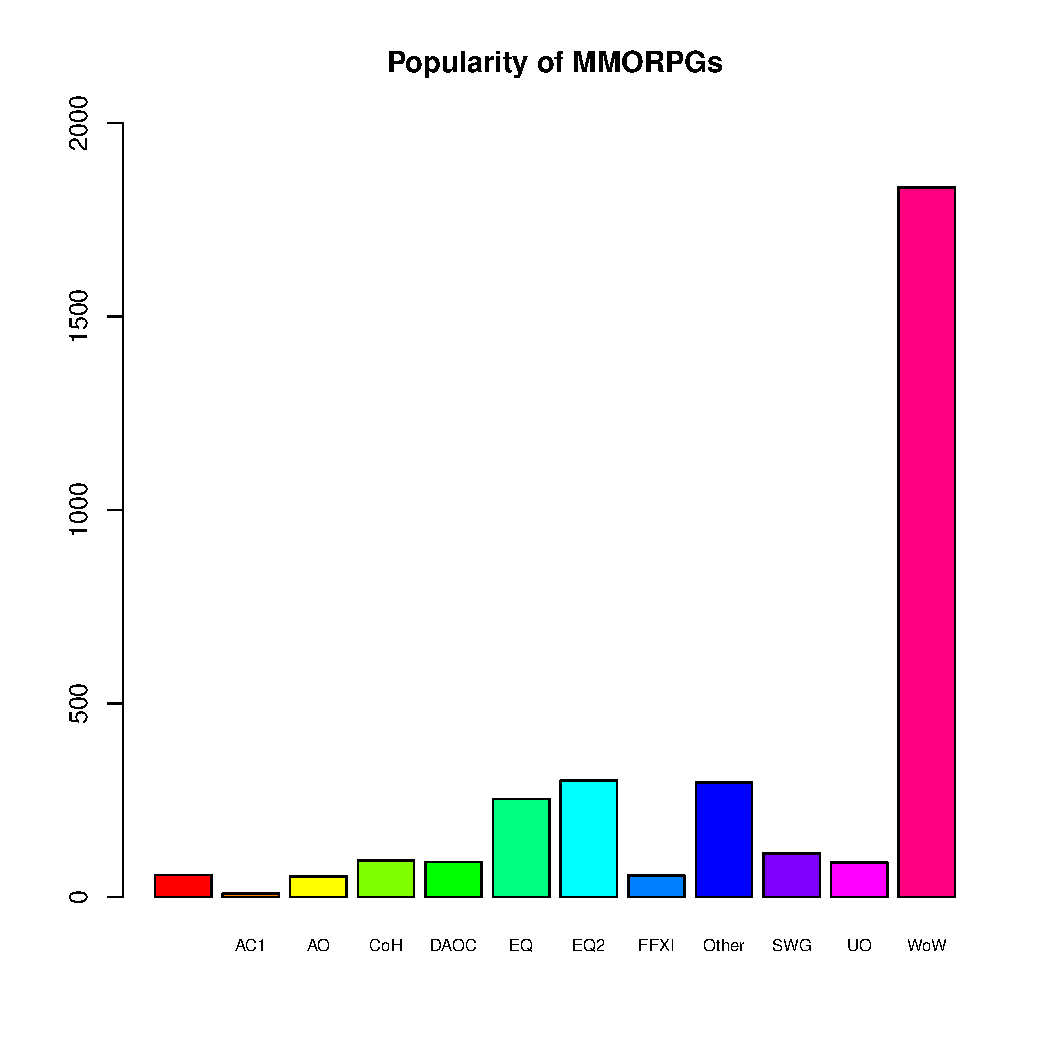
\includegraphics[width=\maxwidth]{figure/unnamed-chunk-11} 
\begin{kframe}\begin{alltt}
\hlkwd{pie}\hlstd{(freqTable}\hlopt{$}\hlstd{relative,}
    \hlkwc{labels} \hlstd{= freqTable}\hlopt{$}\hlstd{Var1,}
    \hlkwc{col}\hlstd{=}\hlkwd{rainbow}\hlstd{(}\hlkwd{length}\hlstd{(freqTable}\hlopt{$}\hlstd{Var1)),}
    \hlkwc{main}\hlstd{=}\hlstr{"Relative popularity of MMORPGs"}\hlstd{)}
\end{alltt}
\end{kframe}
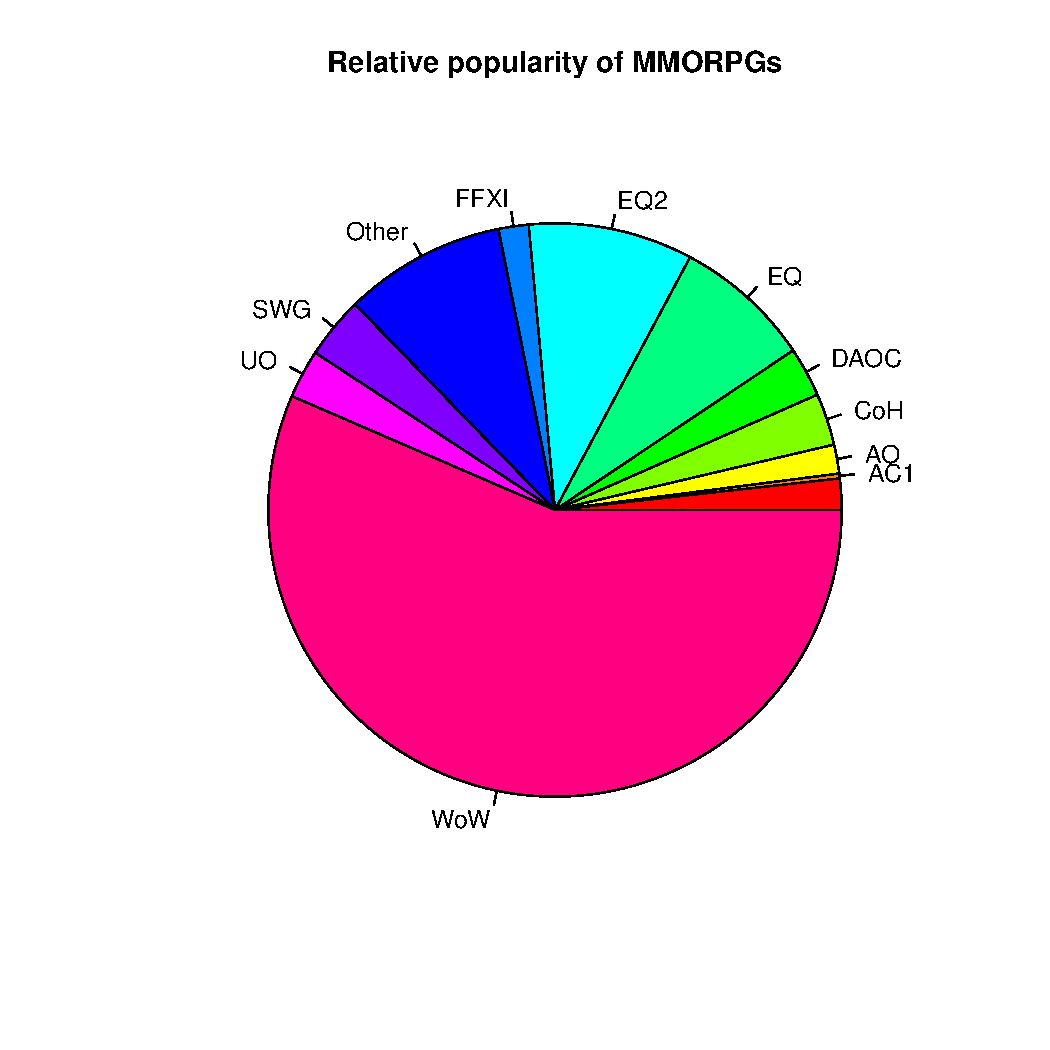
\includegraphics[width=\maxwidth]{figure/unnamed-chunk-12} 

\end{knitrout}


\section{}
\subsection
\emph{What are the top three most popular games?}

\begin{knitrout}
\definecolor{shadecolor}{rgb}{0.969, 0.969, 0.969}\color{fgcolor}\begin{kframe}
\begin{alltt}
\hlkwd{head}\hlstd{(}\hlkwd{sort}\hlstd{(}\hlkwd{table}\hlstd{(}\hlkwd{subset}\hlstd{(data}\hlopt{$}\hlstd{Game, data}\hlopt{$}\hlstd{Game}\hlopt{!=}\hlstr{"Other"}\hlstd{)),}
          \hlkwc{decreasing}\hlstd{=}\hlnum{TRUE}\hlstd{),} \hlkwc{n}\hlstd{=}\hlnum{3}\hlstd{)}
\end{alltt}
\begin{verbatim}
## 
##  WoW  EQ2   EQ 
## 1834  301  253
\end{verbatim}
\end{kframe}
\end{knitrout}



\subsection{}
\emph{What is the proportion of players who played the top three games (do not consider the group Other)? Differentiate separately each proportion of each game by average time spend and gender.}

The column "hours" gives the average hours per week spent playing the game.
Tapply is used to show time spent divided by gender.

\begin{knitrout}
\definecolor{shadecolor}{rgb}{0.969, 0.969, 0.969}\color{fgcolor}\begin{kframe}
\begin{alltt}
\hlstd{wowSet} \hlkwb{=} \hlkwd{subset}\hlstd{(data, data}\hlopt{$}\hlstd{Game} \hlopt{==} \hlstr{"WoW"}\hlstd{)}
\hlstd{eqSet} \hlkwb{=} \hlkwd{subset}\hlstd{(data, data}\hlopt{$}\hlstd{Game} \hlopt{==} \hlstr{"EQ"}\hlstd{)}
\hlstd{eq2Set} \hlkwb{=} \hlkwd{subset}\hlstd{(data, data}\hlopt{$}\hlstd{Game} \hlopt{==} \hlstr{"EQ2"}\hlstd{)}

\hlkwd{tapply}\hlstd{(wowSet}\hlopt{$}\hlstd{Hours, wowSet}\hlopt{$}\hlstd{Gender, mean,} \hlkwc{na.rm} \hlstd{=} \hlnum{TRUE}\hlstd{)}
\end{alltt}
\begin{verbatim}
##        female   male 
##  22.75  26.52  25.15
\end{verbatim}
\begin{alltt}
\hlkwd{tapply}\hlstd{(eqSet}\hlopt{$}\hlstd{Hours, eqSet}\hlopt{$}\hlstd{Gender, mean,} \hlkwc{na.rm} \hlstd{=} \hlnum{TRUE}\hlstd{)}
\end{alltt}
\begin{verbatim}
##        female   male 
##  27.00  24.22  20.67
\end{verbatim}
\begin{alltt}
\hlkwd{tapply}\hlstd{(eq2Set}\hlopt{$}\hlstd{Hours, eq2Set}\hlopt{$}\hlstd{Gender, mean,} \hlkwc{na.rm} \hlstd{=} \hlnum{TRUE}\hlstd{)}
\end{alltt}
\begin{verbatim}
##        female   male 
##  16.80  26.29  21.04
\end{verbatim}
\end{kframe}
\end{knitrout}




\subsection
\emph{On average, which game is played by the youngest gamers and the oldest gamers?}
\begin{knitrout}
\definecolor{shadecolor}{rgb}{0.969, 0.969, 0.969}\color{fgcolor}\begin{kframe}
\begin{alltt}
\hlkwd{sort}\hlstd{(}\hlkwd{tapply}\hlstd{(data}\hlopt{$}\hlstd{Age, data}\hlopt{$}\hlstd{Game, mean,} \hlkwc{na.rm} \hlstd{=} \hlnum{TRUE}\hlstd{),} \hlkwc{decreasing} \hlstd{=} \hlnum{TRUE}\hlstd{)}
\end{alltt}
\begin{verbatim}
##   AC1    EQ  DAOC   CoH    UO   EQ2         SWG    AO   WoW Other  FFXI 
## 35.44 32.24 30.80 30.46 30.45 29.66 29.31 28.39 26.75 26.63 26.00 23.80
\end{verbatim}
\end{kframe}
\end{knitrout}

This shows that the game played by the oldest players is Asheron's Call while Final Fantasy XI has the youngest players on average.


\section{}
\emph{Based on your results, discuss your insights to 
the most popular games.}


As one might expect, MMORPGs are dominated by World of Warcraft. Other games share a relatively similar popularity, only Everquest 1 and 2 are slightly more wide spread. World of Warcraft has six times more players than the second most popular game Everquest 2.

The evaluation of hours spent gaming per week shows that female gamers on average spend more time gaming than male gamers, which contradicts the preconception that play less video games. However the maximum time spent per week is still much higher for male gamers.

The age statistics show that the mean age varies a lot depending on the examined game. The reasons for this remain unclear with the given data - the assumption that it is connected to the release date of the game could not be confirmed. Another assumption could be that the mean age is connected to the supported platforms or specific gameplay mechanics, but this can not be evaluated with the given data.


\section{}
\emph{Based on the provided data, define three networks
based on the dataframe and explain briefly, why 
it might be interesting to analyze existing relations.}
\begin{itemize}
\item
\begin{description}
\item[Vertex]Player
\item[Edge]Teammates
\end{description}
In MMORPGs gamers usually solve quests in small groups and organize themselves in guilds. It would be interesting to see how these relationships compare to the real life and social networks.

\item
\begin{description}
\item[Vertex] Item
\item[Edge] Owned By
\end{description}
When items are traded it would be possible to see how they are distributed. For example it could be possible to identify hubs (traders), or if the items were traded directly. It would also be possible to examine if some items are not used by players regularly but usually sold and then kept by traders. 
\item
\begin{description}
\item[Vertex] Player
\item[Edge] Kill
\end{description}
This relation could provide insight in the way players interact with each other. For example it could be examined if players take revenge after being killed in the game. Another easy evaluation could show if certain players kill or get killed more often than other players. Apart from that it would be interesting to see if kills are evenly distributed or for example restricted to certain fractions in the game.
\end{itemize}
\end{document}
